% !TeX encoding = UTF-8

\chapter{ANÁLISE DOS RESULTADOS}\label{ch:resultados}
Este capítulo tem como finalidade apresentar os resultados obtidos através das implementações demonstradas no Capítulo 5.

\section{ANÁLISE DAS SÉRIES UTILIZADAS}
Após a implementação do modelo da RNA, através dos conjuntos de dados coletados, faz-se necessário avaliar como a respectiva técnica se comportou. Tendo isso em vista, a mesma foi aplicada em função do objetivo principal do trabalho, que é medir a capacidade de precisão de acerto no valor de abertura das ações. Portanto, foi elaborada, de forma independente, uma análise de eficácia do modelo para o cenário de cada empresa utilizada no presente trabalho. É importante ressaltar que os modelos foram implementados levando em consideração todos os \textit{scripts}, métodos e ferramentas utilizadas no capítulo anterior.

\subsection{Aplicação da Rede na Série da Intel Corporation}
A rede da Intel Corporation foi treinada com o objetivo de capturar o maior nível de variação possível dos dados, visando mapear um maior conjunto de padrões e, assim, responder de forma eficiente à dados dispersos através de uma boa capacidade de generalização. Tendo isso em vista, o período de treinamento preparado foi de 09/04/2001 até 21/08/2017, totalizando 4117 registros.

Para o presente caso foram construídos dois cenários de simulação, buscando obter um parâmetro de ciclos de treinamento adequado ao modelo de dados utilizado. As métricas definidas para análise, a partir destes ciclos de treinamento, são: o comportamento da função de custo que compõem o modelo (erro quadrático médio, EQM) e a margem de erro dos valores resultantes da rede, no período de 23/08/2017 a 31/08/2017, em relação aos valores reais. Os parâmetros utilizados foram: 200 e 1000 iterações.

\subsubsection{Treinamento com 200 Iterações}	
A ideia de executar o treinamento com uma quantidade baixa de iterações, é feita com o intuito de proporcionar um treinamento mais rápido e com resultados significativos, levando em consideração as características especificas do modelo de dados. Portanto, para quantificar como ocorreu o processo de treinamento, basta multiplicar o número de iterações (200) com o número de registros de testes (4117), resultando em um total de 823.400 exemplos calculados pela rede. O Gráfico 8 demonstra, de acordo com a quantidade de ciclos, a variação do EQM no primeiro cenário de teste com 200 iterações.
\begin{grafico}[h]
	\centering
	\fbox{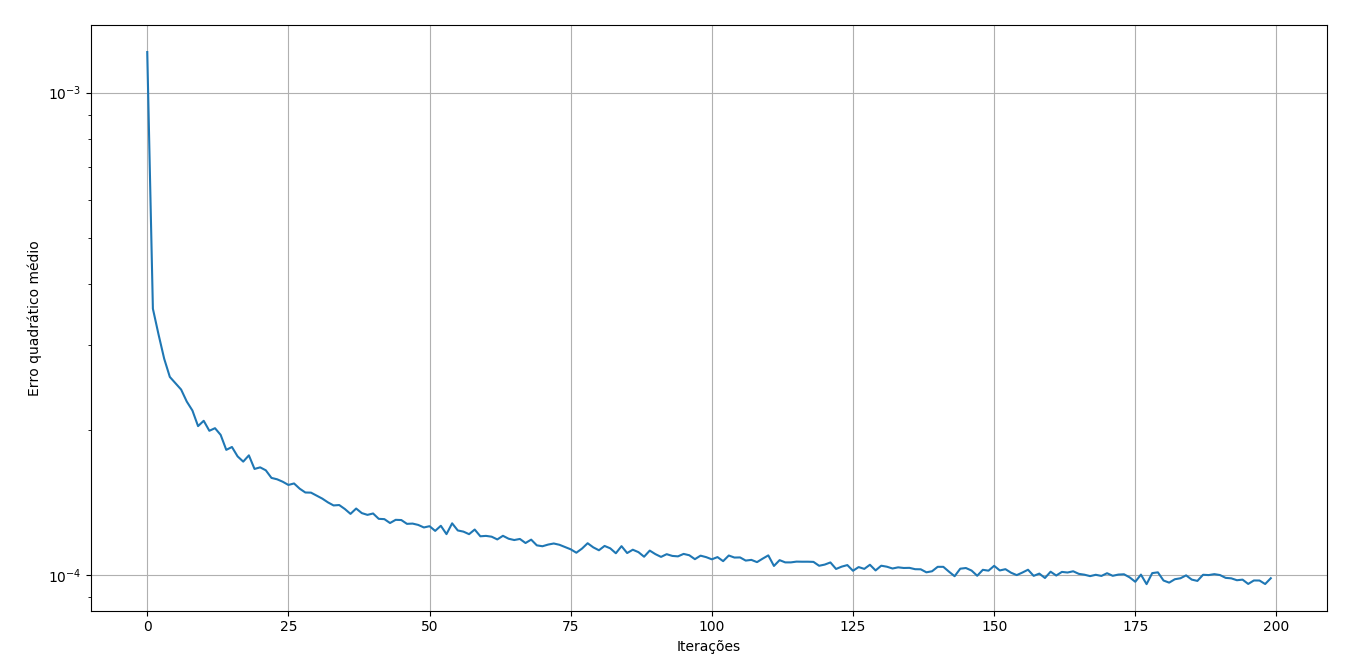
\includegraphics[width=1\textwidth]{erro_intel_primeiro}}
	\caption{Decaimento do EQM no treinamento da rede}
	\fonte{Elaborado pelo autor}
	\label{lingua}
\end{grafico}

O EQM de treinamento iniciou-se, na primeira iteração, com um erro percentual de 0.00248996652176 e, após o término das 200 épocas de treinamento, conclui-se com um erro percentual de 9.44359025338.$10^{-05}$. Analisando o gráfico, pode-se observar que os valores tiveram um decaimento constante até a iteração de número 125, enquanto que, nas 75 iterações posteriores, manteve os valores dos erros aproximados. A queda constante nas iterações iniciais está diretamente ligada a capacidade de aprendizado e adaptação ao modelo de dados.

Tendo em vista a variação dos erros obtidos após a primeira inicialização da rede, foi julgado necessário repetir o mesmo procedimento, visando observar o funcionamento do algoritmo de inicialização dos pesos e validar sua variação aplicada ao mesmo modelo de dados. Portanto, mais dois cenários foram executados com este objetivo. No segundo cenário, o erro foi iniciado com um percentual de 0.00102981131422 e, após o término das 200 épocas de treinamento, concluí-se com um percentual de 9.1790170623.$10^{-05}$. No terceiro cenário, o erro foi iniciado com um percentual de 0.00026991101482 e, após o término das 200 épocas de treinamento, concluí-se com um percentual de 9.49959768553.$10^{-05}$.

Analisando os três cenários, pode-se observar que apesar da rede ser iniciada com os pesos aleatoriamente, o EQM seguiu a mesma tendência para todos os casos, isso implica em uma confiabilidade maior por parte do algoritmo, pois o mesmo garante que novas inicializações, aplicadas ao mesmo modelo de dados, não resultam em valores muito distintos. Esta validação do algoritmo tem grande importância, pois com ela chega-se a definição de que os pesos iniciais da rede não precisarão, necessariamente, serem ajustados manualmente para encontrar um melhor resultado, pois aplicado ao mesmo modelo de dados, os erros seguem o mesmo padrão.

Após a análise do comportamento do EQM e a validação do algortimo de inicialização, os testes foram iniciados com o objetivo de verificar a precisão do modelo. Na Tabela 1 são detalhados os valores do período predito.
\begin{table}[h]
\centering
\caption{Período dos dados utilizados para testes: Intel Corporation}
\vspace{0.5cm}
\begin{tabular}{>{\centering\arraybackslash}m{2cm} >{\centering\arraybackslash}m{2cm} >{\centering\arraybackslash}m{2cm} >{\centering\arraybackslash}m{2cm} >{\centering\arraybackslash}m{2cm} >{\centering\arraybackslash}m{2cm}}
\toprule
Data    & Abertura   & Alta   & Baixa   & Fechamento   & Volume\\
\midrule
23/08/2017 & 34.54 & 34.81 & 34.38 & 34.66 & 196.481,34\\
24/08/2017 & 34.70 & 34.89 & 34.55 & 34.71 & 143.018,92\\
25/08/2017 & 34.82 & 34.93 & 34.58 & 34.67 & 147.268,29\\
28/08/2017 & 34.78 & 34.80 & 34.59 & 34.65 & 207.128,76\\
29/08/2017 & 34.51 & 34.75 & 34.46 & 34.73 & 158.436,68\\
30/08/2017 & 34.75 & 34.96 & 34.63 & 34.89 & 185.650,07\\
31/08/2017 & 34.94 & 35.18 & 34.87 & 35.07 & 163.667,72\\
\bottomrule
\end{tabular}
\end{table}

Os dados demonstrados na Tabela 1 foram refinados e normalizados de acordo com os métodos implementados no Capítulo 5. Após a execução deste processo, os mesmos foram inseridos na RNA para ativação. Posteriormente, foi realizada a desnormalização e os resultados apresentados. A Tabela 2 ilustra os resultados obtidos.
\begin{table}[h]
\centering
\caption{Resultados da predição realizada nos dados utilizados pela rede}
\vspace{0.5cm}
\begin{tabular}{>{\centering\arraybackslash}m{2cm} >{\centering\arraybackslash}m{2cm} >{\centering\arraybackslash}m{2cm} >{\centering\arraybackslash}m{2cm} >{\centering\arraybackslash}m{2cm}}
\toprule
Data    & Valor real   & Resultado    & Erro (\%) & Variação\\
\midrule
23/08/2017 & 34.54 & 34.73 & 0.550 & -0.19\\
24/08/2017 & 34.70 & 34.71 & 0.028 & -0.01\\
25/08/2017 & 34.82 & 34.79 & 0.086 & 0.03\\
28/08/2017 & 34.78 & 34.77 & 0.028 & 0.01\\
29/08/2017 & 34.51 & 34.75 & 0.695 & -0.24\\
30/08/2017 & 34.75 & 34.82 & 0.201 & -0.07\\
31/08/2017 & 34.94 & 34.99 & 0.143 & 0.05\\
\bottomrule
\end{tabular}
\end{table}

Analisando a Tabela 2, pode-se observar que os resultados obtidos foram significativos, onde o percentual de erro calculado, através do erro relativo percentual, não ultrapassou a margem 0.70\%, se aproximando, consideravelmente, dos valores reais. O erro médio, analisado para todo o período de predição, ficou em torno de 0.24\%, o que pode ser considerado baixo levando-se em conta o número de iterações utilizadas para treinar a RNA. Já a medida de dispersão dos erros em torno da média obtida (desvio padrão) foi de aproximadamente 0.26\%. Entretanto, analisando de forma mais detalhada cada valor resultante, pode-se evidenciar dois erros mais altos nos dias 23/08/2017 e 29/08/2017, com 0.550\% e 0.695\%, respectivamente. Tendo em vista que os valores mais próximos aos verdadeiros oscilaram no intervalo entre [34.70, 34.82], fica evidente que o modelo obteve erros mais altos em momentos de queda no valor desta série. A ocorrência destes erros acontece através da tendência de padrões em que a rede foi treinada, de forma crescente, não acompanhando assim as quedas bruscas no período. Isto fica mais claro observando o valor predito do dia 31/08/2017, onde o valor real obteve uma alta considerável, se comparada aos valores anteriores, porém não afetou a capacidade de precisão da RNA, mantendo a margem de erro pequena. O Gráfico 9 representa, de maneira ilustrativa, os resultados da série.
\begin{grafico}[h]
	\centering
	\fbox{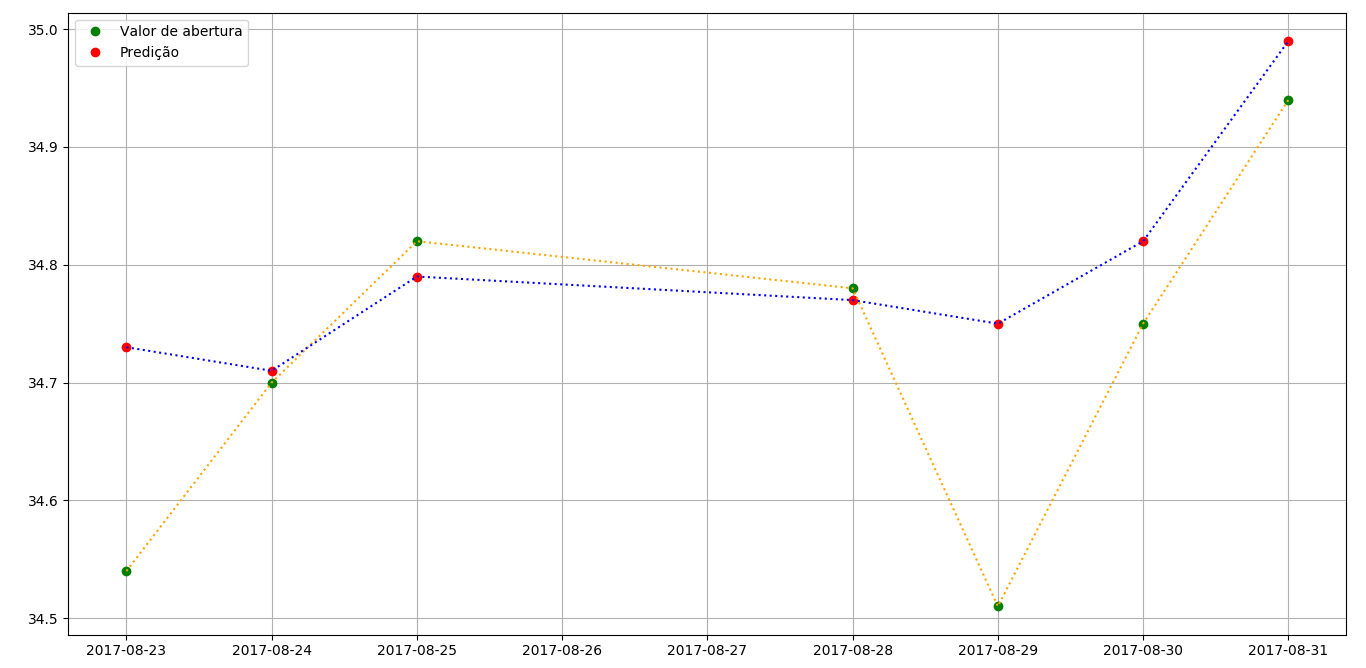
\includegraphics[width=1\textwidth]{predicao_intel}}
	\caption{Distribuição dos dados resultantes da RNA e seus valores esperados}
	\fonte{Elaborado pelo autor}
	\label{lingua}
\end{grafico}

Analisando o gráfico é possível observar como os resultados são próximos aos esperados. Os valores de abertura, nos respectivos dias testados, são representados por um ponto verde. Já os resultados obtidos pela rede são caracterizados pelo ponto vermelho. No Gráfico também fica evidente, de maneira ilustrativa, como a série não acompanhou as quedas do período e seguiu uma tendência crescente. 

\subsubsection{Treinamento com 1000 Iterações}	
Com a finalidade de comparar com a simulação anterior, foi realizado um teste com 1000 épocas de treinamento visando alcançar um resultado mais preciso e, também, para validar se o aumento na quantidade de iterações, no processo de treinamento, melhoram os resultados retornados pela rede.

Para quantificar como ocorreu o processo de treinamento, basta multiplicar o número de iterações (1000) com o número de registros de testes (4117), resultando em um total de 4.117.000 exemplos calculados pela rede.

Para o primeiro cenário a rede iniciou-se, na primeira iteração, com um erro percentual de 0.00664064049629 e, após o término das 1000 épocas de treinamento, conclui-se com um erro percentual de 8.7943563121853531.$10^{-05}$. Mais dois treinos distintos foram realizados visando encontrar alguma dispersão no erro obtido pela rede, como feito na análise anterior. Portanto, o segundo treino obteve um erro inicial de 0.00260377914122 e, após o término das 1000 épocas de treinamento, conclui-se com um percentual de 8.91402403614.$10^{-05}$. O terceiro treino obteve um erro inicial de 0.00496238079711 e, após o término das 1000 épocas de treinamento, o EQM do treinamento conclui-se com um percentual de 8.90814371631.$10^{-05}$.

Após a execução desses cenários de treinamento, pode-se concluir que a rede se comportou de forma estável em relação a quantidade de iterações, não distinguindo, de forma relevante, os valores dos pesos em diversas inicializações aleatórias. O Gráfico 10 representa, de maneira ilustrativa, o comportamento do EQM da rede treinada pelo primeiro cenário.
\begin{grafico}[h]
	\centering
	\fbox{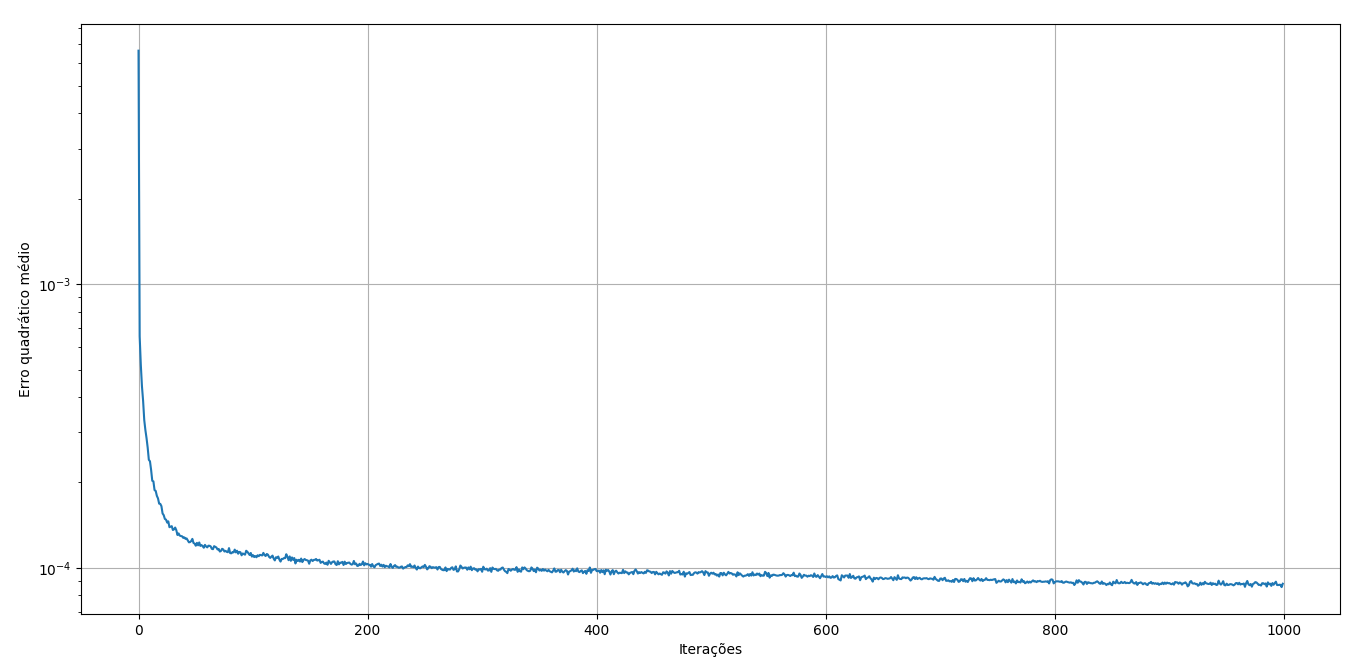
\includegraphics[width=1\textwidth]{erro_intel_1000iteracoes}}
	\caption{Decaimento do EQM no treinamento da rede}
	\fonte{Elaborado pelo autor}
	\label{lingua}
\end{grafico}

Analisando o Gráfico 10, pode-se observar que o erro obteve uma queda constante até 200 iterações, enquanto que, entre as iterações de número 200 até a de número 400, manteve o padrão com valores aproximados. Os últimos 600 ciclos mantiveram um decaimento mínimo do EQM.

Tendo em vista a simulação anterior, com 200 iterações, fica claro que a queda brusca e rápida aconteceria nas primeiras iterações, pois a base de dados utilizada é a mesma. Também é possível observar, através de um número maior de iterações, que o EQM obteve resultados mais baixos em comparação ao treino anterior.

O período aplicado para a realização dos testes foi o mesmo utilizado da Tabela 1. Os dados foram devidamente refinados, normalizados e, a partir disto, foram ativados na rede. Os resultados preditos, a partir da execução dos testes, são demonstrados na Tabela 3.
\begin{table}[h]
\centering
\caption{Resultados da predição realizada nos dados utilizados pela rede}
\vspace{0.5cm}
\begin{tabular}{>{\centering\arraybackslash}m{2cm} >{\centering\arraybackslash}m{2cm} >{\centering\arraybackslash}m{2cm} >{\centering\arraybackslash}m{2cm} >{\centering\arraybackslash}m{2cm}}
\toprule
Data    & Valor real   & Resultado    & Erro (\%) & Variação\\
\midrule
23/08/2017 & 34.54 & 34.67 & 0.376 & -0.13\\
24/08/2017 & 34.70 & 34.64 & 0.172 & 0.06\\
25/08/2017 & 34.82 & 34.71 & 0.315 & 0.11\\
28/08/2017 & 34.78 & 34.68 & 0.287 & 0.10\\
29/08/2017 & 34.51 & 34.65 & 0.405 & -0.14\\
30/08/2017 & 34.75 & 34.70 & 0.143 & 0.05\\
31/08/2017 & 34.94 & 34.84 & 0.286 & 0.10\\
\bottomrule
\end{tabular}
\end{table}

Analisando a Tabela 3, pode-se observar que os resultados obtidos foram significativos, onde o percentual de erro calculado, através do erro relativo percentual, não ultrapassou a margem 0.50\%, se aproximando consideravelmente dos valores reais. O erro médio, de todo o período analisado, obteve um valor de aproximadamente 0.28\%, superior ao treinamento anterior. Já a medida de dispersão dos erros em torno da média obtida (desvio padrão) foi de aproximadamente 0.09\%. Sendo assim, pode-se concluir que o desvio padrão foi menor que o do primeiro cenário, devido ao fato dos erros mais altos (23/08/2017 e 29/08/2017) serem mais suaves. O Gráfico 11 representa, de maneira ilustrativa, os resultados da rede.

\begin{grafico}[h]
	\centering
	\fbox{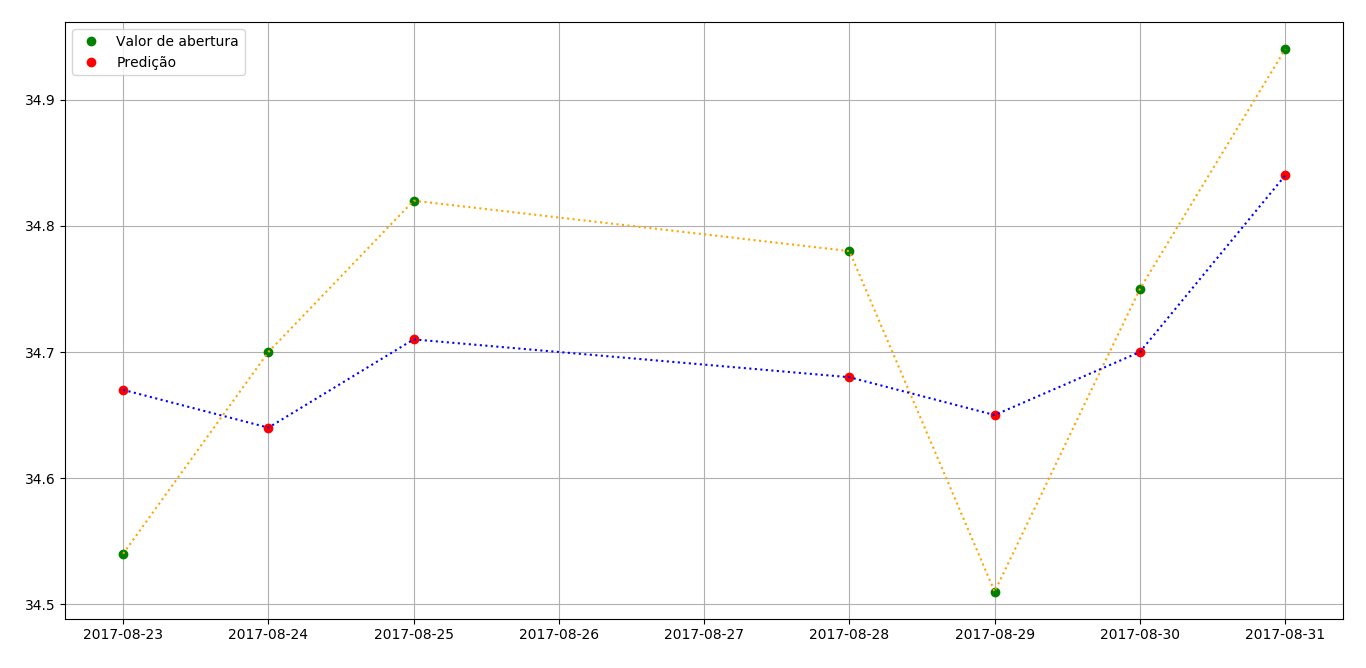
\includegraphics[width=1\textwidth]{predicao_intel_1000}}
	\caption{Distribuição dos dados resultantes da RNA e seus valores esperados}
	\fonte{Elaborado pelo autor}
	\label{lingua}
\end{grafico}

Apesar da diferença do erro percentual relativo entre os dois cenários ser de apenas 4\%, foi encontrada uma melhor parâmetrização para o presente modelo de dados utilizando um treinamento com 200 iterações, pois a exatidão dos valores preditos foram mais eficazes neste método de treinamento. Sendo assim, chega-se a definição que nem sempre um número maior de ciclos de treinamento aumentam a precisão da RNA. Neste caso, a rede sofreu uma convergência do EQM em torno de 200 iteraçoes, este detalhe pode ser observado visualizando o comportamento do Gráfico 10. Dessa forma, as iterações posteriores propagaram o erro de forma desnecessária, alterando assim os pesos sinápticos dos neurônios e, automaticamente, causando uma maior dispersão nos resultados. Este processo ocorrido na segunda simulação, na literatura, é denominado \textit{Overtraining}, detalhado no Capítulo 3.

\subsection{Aplicação da Rede na Série da Microsoft Corporation}
A rede da Microsoft Corporation foi treinada utilizando as mesmas técnicas da Intel Corporation, ou seja, com o intuito de capturar o maior nível de variação possível dos dados, visando mapear um maior conjunto de padrões e, assim, obter uma boa capacidade de generalização. Tendo isso em vista, o período de treinamento preparado foi de 09/04/2001 até 21/08/2017, totalizando 4117 registros.

Para o presente caso foram construídos dois cenários de simulação, buscando obter um parâmetro de ciclos de treinamento adequado ao modelo de dados utilizado. As métricas definidas para análise, a partir destes ciclos de treinamento, são: o comportamento da função de custo que compõem o modelo (erro quadrático médio, EQM) e a margem de erro dos valores resultantes da rede, no período de 23/08/2017 a 31/08/2017, em relação aos valores reais. Os parâmetros de ciclos de treinamento utilizados foram: 200 e 1000 iterações.

\subsubsection{Treinamento com 200 Iterações}	
O treinamento com 200 iterações foi executado com o objetivo de verificar a capacidade de precisão da rede com um número menor de iterações. Para quantificar como ocorreu o processo de treinamento, basta multiplicar o número de iterações (200) com o número de registros de testes (4117), resultando em um total de 823.400 exemplos calculados pela rede.

Para este caso, a RNA foi inicializada duas vezes com o objetivo de observar o comportamento e a tendência do EQM em relação ao algoritmo de inicialização. No primeiro cenário, a rede iniciou-se com o EQM em 0.0018579672451418453 e, após as 200 iterações, conclui-se com um erro de 3.6623220378015219.$10^{-05}$. No segundo cenário, o erro foi inicializado com 0.0047598765727053707 e, após as 200 iterações, conclui-se com um erro de 3.8483854181673219.$10^{-05}$.

É possível verificar, através dos dois cenários executados, que o erro seguiu a mesma tendência para os dois casos, com um erro final próximo a 3.$10^{-05}$. Tendo isso em vista, possíveis inicializações distintas, aplicada ao modelo de dados da Microsoft Corporation, não irão resultar em valores muito distintos pois a diferença do erro é mínima.

Para demonstrar, de maneira mais clara, o comportamento do erro obtido pela rede em todo processo de treinamento, o Gráfico 12 demonstra, de acordo com a quantidade ciclos, a variação do EQM no primeiro cenário de teste.
\begin{grafico}[h]
	\centering
	\fbox{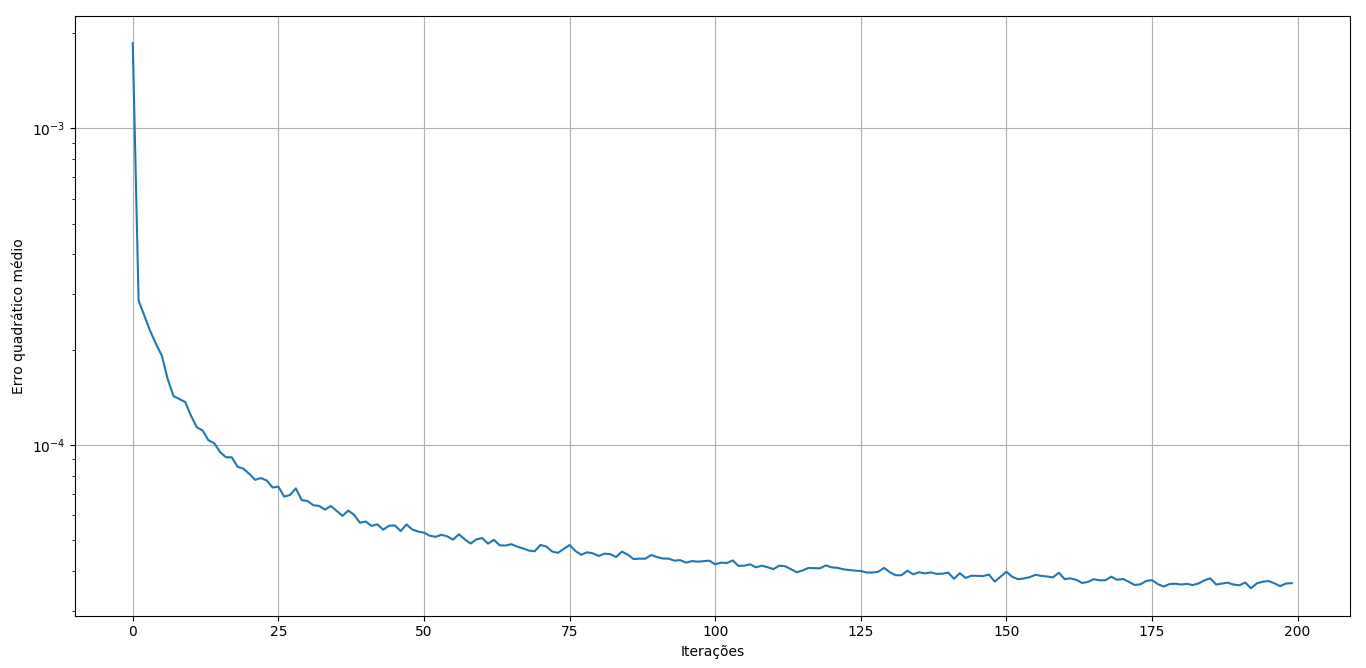
\includegraphics[width=1\textwidth]{erro_microsoft_200_segundo_cenario}}
	\caption{Decaimento do EQM no treinamento da rede}
	\fonte{Elaborado pelo autor}
	\label{lingua}
\end{grafico}

Analisando o gráfico, pode-se observar que os valores tiveram um decaimento constante até a iteração de número 125, enquanto que, nas 75 iterações posteriores, manteve os valores dos erros aproximados. A queda constante nas iterações iniciais está diretamente ligada a capacidade de aprendizado e adaptação ao modelo de dados.

Após a análise do comportamento do EQM e a validação do algortimo de inicialização, os testes foram iniciados com o objetivo de verificar a precisão do modelo. Na Tabela 4 são detalhados os valores do período predito.
\begin{table}[h]
\centering
\caption{Período dos dados utilizados para testes: Microsoft Corporation}
\vspace{0.5cm}
\begin{tabular}{>{\centering\arraybackslash}m{2cm} >{\centering\arraybackslash}m{2cm} >{\centering\arraybackslash}m{2cm} >{\centering\arraybackslash}m{2cm} >{\centering\arraybackslash}m{2cm} >{\centering\arraybackslash}m{2cm}}
\toprule
Data    & Abertura   & Alta   & Baixa   & Fechamento   & Volume\\
\midrule
23/08/2017 & 72.96 & 73.15 & 72.53 & 72.72 & 137.665,07\\
24/08/2017 & 72.74 & 72.86 & 72.07 & 72.69 & 170.982,82\\
25/08/2017 & 72.86 & 73.35 & 72.48 & 72.82 & 127.943,01\\
28/08/2017 & 73.06 & 73.09 & 72.55 & 72.83 & 145.697,15\\
29/08/2017 & 72.25 & 73.16 & 72.05 & 73.05 & 114.783,82\\
30/08/2017 & 73.01 & 74.21 & 72.83 & 74.01 & 168.978,01\\
31/08/2017 & 74.03 & 74.96 & 73.80 & 74.77 & 276.528,11\\
\bottomrule
\end{tabular}
\end{table}

Os dados demonstrados na Tabela 4 foram refinados e normalizados de acordo com os métodos implementados no Capítulo 5. Após a execução deste processo, os mesmos foram inseridos na RNA para ativação. Posteriormente, foi realizada a desnormalização e os resultados apresentados. Na tabela 5 é possível verificar os resultados obtidos pela rede.

\begin{table}[h]
\centering
\caption{Resultados da predição realizada nos dados utilizados pela rede}
\vspace{0.5cm}
\begin{tabular}{>{\centering\arraybackslash}m{2cm} >{\centering\arraybackslash}m{2cm} >{\centering\arraybackslash}m{2cm} >{\centering\arraybackslash}m{2cm} >{\centering\arraybackslash}m{2cm}}
\toprule
Data    & Valor real   & Resultado    & Erro (\%) & Variação\\
\midrule
23/08/2017 & 72.96 & 72.94 & 0.027 & 0.02\\
24/08/2017 & 72.74 & 72.61 & 0.028 & 0.13\\
25/08/2017 & 72.86 & 72.50 & 0.086 & 0.36\\
28/08/2017 & 73.06 & 72.73 & 0.028 & -0.33\\
29/08/2017 & 72.25 & 72.64 & 0.695 & -0.39\\
30/08/2017 & 73.01 & 72.82 & 0.201 & 0.19\\
31/08/2017 & 74.03 & 73.75 & 0.143 & 0.28\\
\bottomrule
\end{tabular}
\end{table}

Analisando a Tabela 5, pode-se observar que os resultados obtidos foram significativos, onde o percentual de erro calculado, através do erro relativo percentual, não ultrapassou a margem 0.70\%, se aproximando, consideravelmente, dos valores reais. O erro médio, analisado para todo o período de predição, ficou em torno de 0.17\%, o que pode ser considerado baixo levando-se em conta o número de iterações utilizadas para treinar a RNA. Já a medida de dispersão dos erros em torno da média obtida (desvio padrão) foi de aproximadamente 0.23\%. O Gráfico 13 detalha, de forma ilustrativa, o comportamento dos resultados esperados e os resultados alcançados pela RNA.
\begin{grafico}[h]
	\centering
	\fbox{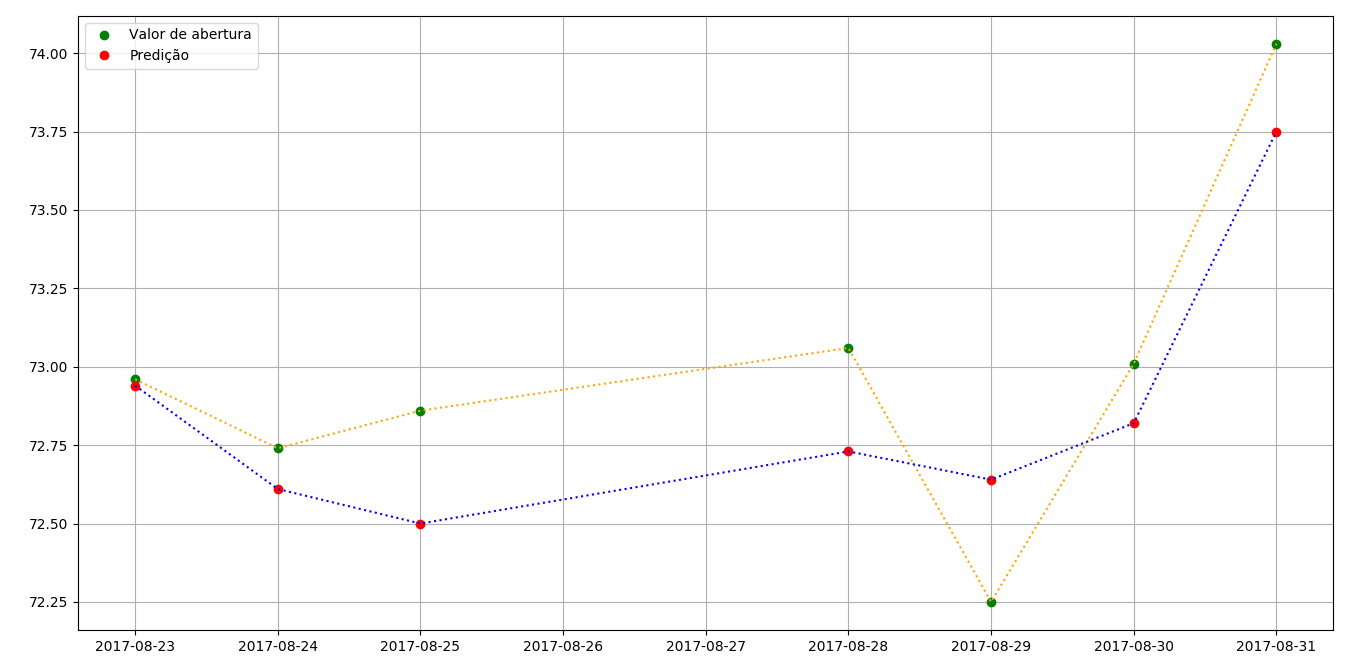
\includegraphics[width=1\textwidth]{microsoft_resultados}}
	\caption{Distribuição dos dados resultantes da RNA e seus valores esperados}
	\fonte{Elaborado pelo autor}
	\label{lingua}
\end{grafico}

Visualizando os erros obtidos, pode-se evidenciar que não houve grande dispersão no período, com excessão do dia 29/08/2017, que foi o mais alto de toda a série. Este erro foi o mais alto porque houve uma queda grande no valor da ação, se comparado ao padrão que a mesma vinha seguindo. Seguindo esta linha de análise, é preciso destacar que houve um aumento significativo no valor da ação, mais especificamente no dia 31/08/2017, porém, diferentemente do momento de queda, a rede se adaptou a este acrescimento e suavizou o erro. 

A partir destes cenários levantados, é possível chegar a conclusão de que a rede não conseguiu prever com mais exatidão os momentos de queda da ação, enquanto que, nos momentos de alta, obteve uma boa capacidade de adaptabilidade.

\subsubsection{Treinamento com 1000 Iterações}	
Com a finalidade de comparar com a simulação anterior, foi realizado um teste com 1000 épocas de treinamento visando alcançar um resultado mais preciso e, também, para validar se o aumento na quantidade de iterações, no processo de treinamento, melhoram os resultados retornados pela rede.

Para quantificar como ocorreu o processo de treinamento, basta multiplicar o número de iterações (1000) com o número de registros de testes (4117), resultando em um total de 4.117.000 exemplos calculados pela rede.

Para o primeiro cenário a rede iniciou-se, na primeira iteração, com um erro percentual de 0.005757041736 e, após o término das 1000 épocas de treinamento, conclui-se com um erro percentual de 3.0266887029028769.$10^{-05}$. Mais dois treinos distintos foram realizados visando encontrar alguma dispersão no erro obtido pela rede, como feito na análise anterior. Portanto, o segundo treino obteve um erro inicial de 0.0035660777044 e, após o término das 1000 épocas de treinamento, conclui-se com um percentual de 2.57225977588.$10^{-05}$. O terceiro treino obteve um erro inicial de 0.00624617417834 e, após o término das 1000 épocas de treinamento, o EQM do treinamento conclui-se com um percentual de 2.5743685343480545.$10^{-05}$.
\begin{grafico}[h]
	\centering
	\fbox{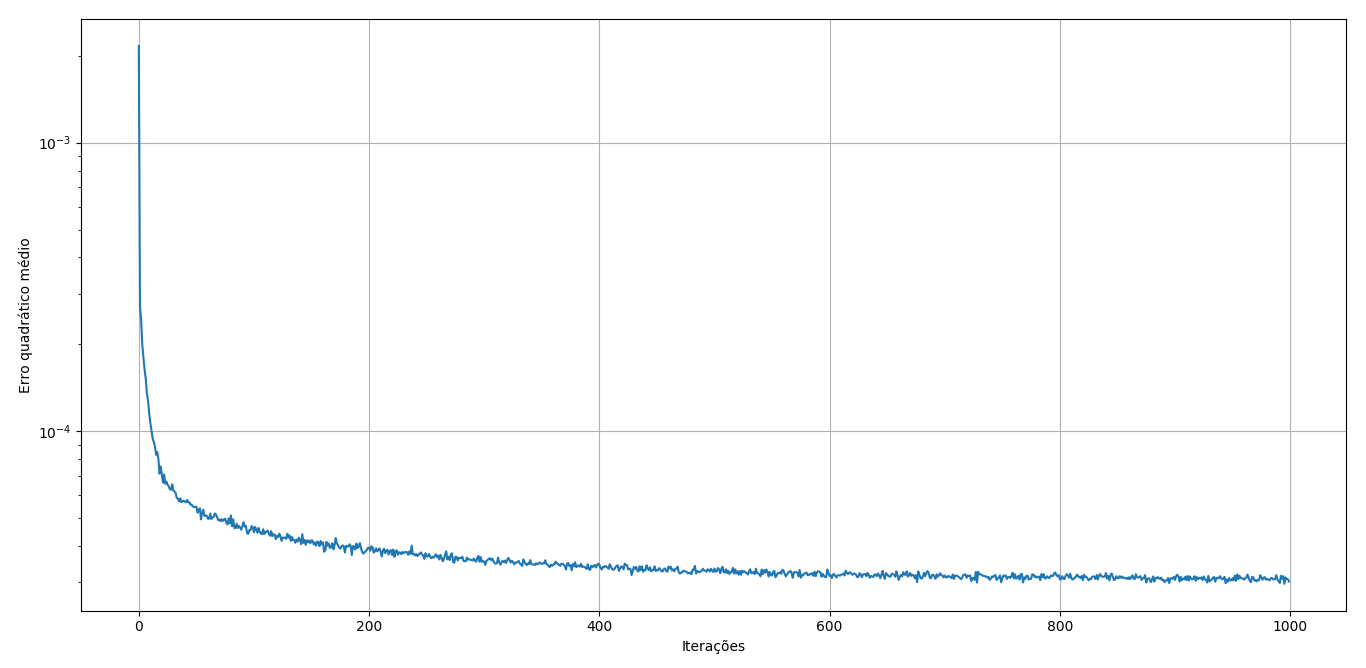
\includegraphics[width=1\textwidth]{erro_microsoft_1000}}
	\caption{Decaimento do EQM no treinamento da rede}
	\fonte{Elaborado pelo autor}
	\label{lingua}
\end{grafico}

Analisando o Gráfico 14, que representa a variação do EQM no primeiro cenário de teste iniciado, pode-se observar que o mesmo obteve uma queda constante até 600 iterações, enquanto que, entre as iterações de número 600 até a de número 1000, manteve o padrão com valores aproximados, ou seja, foi o momento em que a RNA convergiu. 

Portanto, após a execução desses cenários de treinamento, analisando o comportamento do peso e a sua variação, pode-se concluir que o modelo se comportou de forma estável, não distinguindo, de forma relevante, os valores dos pesos em diversas inicializações aleatórias.

A partir disso, é possível assegurar que o algoritmo de inicialização não vai influenciar em resultados diferentes, caso várias inicializações distintas sejam executadas ao mesmo modelo de dados. 

Após a observação do comportamento do erro, o período de teste (Tabela 4) foi inserido na rede. Os dados foram devidamente refinados, normalizados e, a partir disso, foram ativados. Os resultados preditos, a partir da execução dos testes, são demonstrados na Tabela 6. 

\begin{table}[h]
\centering
\caption{Resultados da predição realizada nos dados utilizados pela rede}
\vspace{0.5cm}
\begin{tabular}{>{\centering\arraybackslash}m{2cm} >{\centering\arraybackslash}m{2cm} >{\centering\arraybackslash}m{2cm} >{\centering\arraybackslash}m{2cm} >{\centering\arraybackslash}m{2cm}}
\toprule
Data    & Valor real   & Resultado    & Erro (\%) & Variação\\
\midrule
23/08/2017 & 72.96 & 72.73 & 0.315 & 0.23\\
24/08/2017 & 72.74 & 72.51 & 0.316 & 0.23\\
25/08/2017 & 72.86 & 72.37 & 0.672 & 0.49\\
28/08/2017 & 73.06 & 72.60 & 0.629 & 0.46\\
29/08/2017 & 72.25 & 72.59 & 0.470 & -0.34\\
30/08/2017 & 73.01 & 72.58 & 0.588 & 0.43\\
31/08/2017 & 74.03 & 73.45 & 0.783 & 0.58\\
\bottomrule
\end{tabular}
\end{table}

Analisando a Tabela 6, pode-se observar que os resultados sofreram uma maior dispersão, se comparado ao treinamento anterior. O percentual de erro calculado, através do erro relativo percentual, não ultrapassou a margem 0.80\%. A média de todo o período analisado obteve um erro de de aproximadamente 0.53\%, superior a média do treinamento anterior. Já a medida de dispersão dos erros em torno da média obtida (desvio padrão) foi de aproximadamente 0.17\%.

No presente cenário em análise, o valor mais falho de toda a série foi o do dia 31/08/2017. Comparando-o com o resultado de 200 iterações, pode-se observar que a rede perdeu a capacidade de adaptabilidade para prever momentos de alta na ação, após o aumento na quantidade de épocas de treinamento. Observando o segundo maior erro da série, obtido no dia 25/08/2017, pode-se notar que o mesmo se encontra dentro dos padrões de tendência em que a rede vinha seguindo, porém a RNA também corrompeu o resultado predito. Este embaralhamento nos resultados mais uma vez está ligado a capacidade de convergência da RNA, onde, após convergir em uma quantidade menor de iterações, as épocas posteriores apenas propagaram o erro desnecessariamente, modificando os pesos sinápticos dos neurônios da camada oculta com valores desnecessários e, assim, causando instabilidade na capacidade de precisão do modelo aplicado. 

Portanto, novamente é possível observar que o aumento na quantidade de épocas de treinamento e a diminuição do EQM, não necessariamente implicam em uma capacidade maior de previsão e generalização da RNA. No Gráfico 15 é possível notar, de forma mais intuitiva, em quais momentos a previsão obteve maior e menor exatidão, levando em consideração os pontos dos valores reais da ação analisada.

\begin{grafico}[h]
	\centering
	\fbox{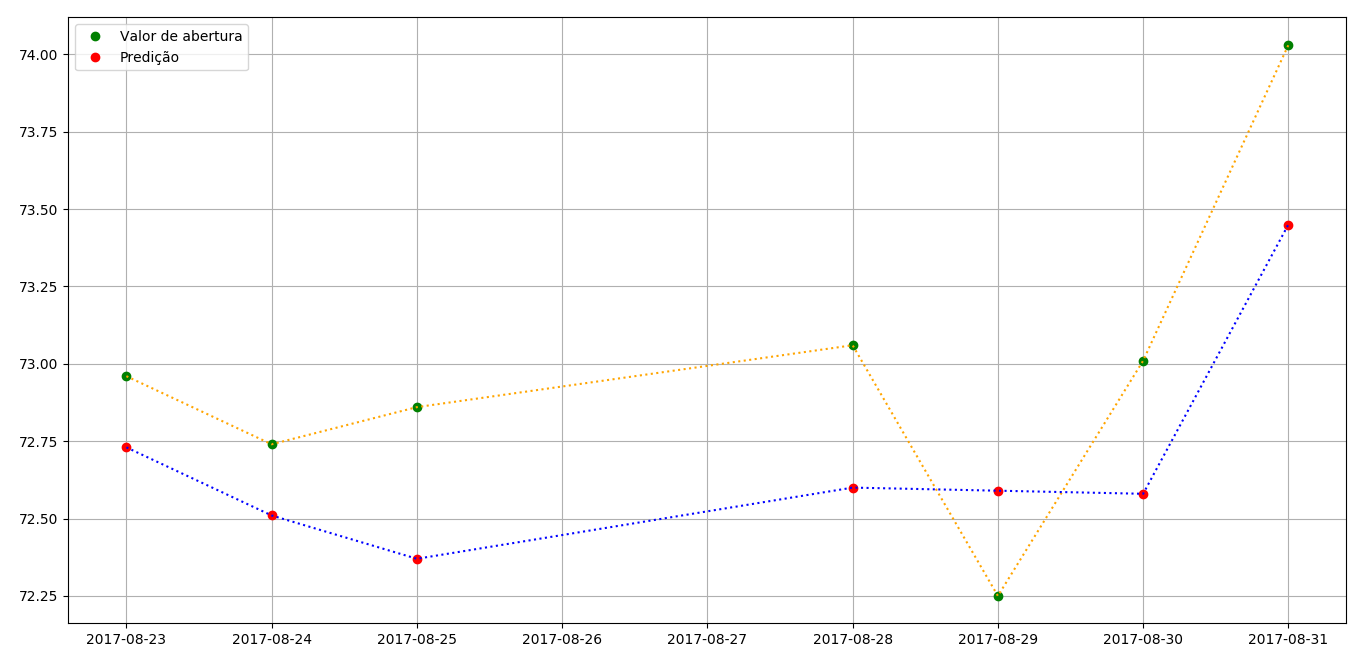
\includegraphics[width=1\textwidth]{microsoft_1000_resultado}}
	\caption{Distribuição dos dados resultantes da RNA e seus valores esperados}
	\fonte{Elaborado pelo autor}
	\label{lingua}
\end{grafico}

\subsection{Aplicação da Rede na Série da Apple Inc}
A rede da Apple foi treinada utilizando as mesmas técnicas dos cenários anteriormente testados, ou seja, com o intuito de capturar o maior nível de variação possível dos dados, proporcionando para a RNA mapear uma quantia significativa de valores e situações distintas, presentes na série histórica utilizada, além de buscar uma boa capacidade de generalização para o modelo aplicado. O período de treinamento preparado foi de 09/04/2001 até 21/08/2017, totalizando 4117 registros.

Para o presente caso foram construídos dois cenários de simulação, buscando obter um parâmetro de ciclos de treinamento adequado ao modelo de dados utilizado. As métricas definidas para análise, a partir destes ciclos de treinamento, são: o comportamento da função de custo que compõem o modelo (erro quadrático médio, EQM) e a margem de erro dos valores resultantes da rede, no período de 23/08/2017 a 31/08/2017, em relação aos valores reais. Os parâmetros de ciclos de treinamento utilizados foram: 200 e 1000 iterações.

\subsubsection{Treinamento com 200 Iterações}	
O treinamento com 200 iterações foi executado com o objetivo de verificar a capacidade de precisão da rede com um número menor de iterações. Para quantificar como ocorreu o processo de treinamento, basta multiplicar o número de iterações (200) com o número de registros de testes (4117), resultando em um total de 823.400 exemplos calculados pela rede.

Para este caso, a RNA foi inicializada duas vezes com o objetivo de observar o comportamento e a tendência do EQM em relação ao algoritmo de inicialização. No primeiro cenário, a rede iniciou-se com o EQM em 0.000439745663518 e, após as 200 iterações, conclui-se com um erro de 1.9971768385490857.$10^{-05}$. No segundo cenário, o erro foi inicializado com 0.000710657880333 e, após as 200 iterações, conclui-se com um erro de 1.915103371487409.$10^{-05}$. O Gráfico x demonstra, de forma mais intuitiva, o comportamento do EQM no primeiro cenário de inicialização e treinamento da rede.
\begin{grafico}[h]
	\centering
	\fbox{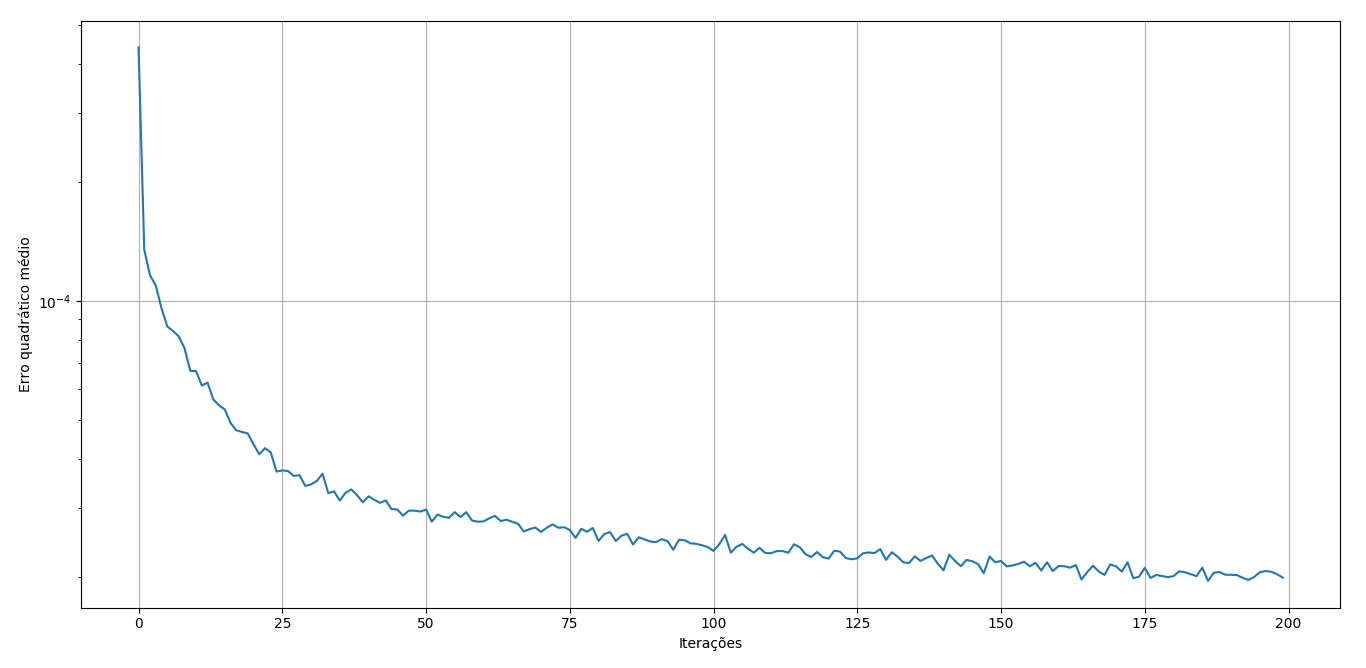
\includegraphics[width=1\textwidth]{erro_apple_200}}
	\caption{Decaimento do EQM no treinamento da rede}
	\fonte{Elaborado pelo autor}
	\label{lingua}
\end{grafico}

É possível verificar, através dos dois cenários executados, que o erro seguiu a mesma tendência para os dois casos, com um erro final próximo a 1.$10^{-05}$. Tendo isso em vista, possíveis inicializações distintas, aplicada ao modelo de dados da Apple Inc, não irão resultar em valores muito distintos pois a diferença do erro é mínima.